\section{Ejercicio 1}

\subsection{Introducción}

\paragraph{}
El primer problema del presente trabajo consistió en la implementación de un algoritmo capaz de dar solución a la ecuación 
	\begin{equation} 
		b^n\ mod\ (n)
	\label{problema}
	\end{equation}
haciendo uso de alguna de las técnicas algorítmicas aprendidas hasta el momento en la materia. Asímismo, la consigna dictaba que la complejidad final del algoritmo debería ser menor a \Ode{n}.\\

\paragraph{}
En pos de cumplimentar lo pedido se decidió usar la técnica de \textit{Dividir \& Conquistar}\footnote{Poner alguna referencia 	en donde se explique esta técnica} para desarrollar el algoritmo. Esta técnica se caracteriza principalmente en dividir la instancia de un problema en instancias más pequeñas, atacar cada una de ellas por separado y resolverlas, para finalmente juntar sus resultados y así producir el resultado final.

\subsection{Explicación}

\paragraph{}
La primera solución que se piensa casi de manera intuitiva es la de mutliplicar \textit{n} veces el número \textit{b} y luego hallar el resto de dividir ese resultado por \textit{n}. 
	\begin{equation}
		\underbrace{b.b.b \hdots b.b.b}_{n\ veces}\ mod\ (n)  = b^n\ mod\ (n)
	\label{primera_idea}		
	\end{equation}
Sin embargo, la complejidad ese algoritmo es \Ode{n}, ya que se realizan \textit{n} multipicaciones y 1 división, razón por lo cual no cumple con lo pedido en la consigna. Además, puesto que ese algoritmo realizar sucesivas multipliciones de \textit{b}, cabe la posibilidad de que el valor en que se va acumulando el resultado sobrepase el máximo número entero representable en la computadora produciedo así un overflow y obteniéndose en consecuencia un resultado incorrecto. \\

\paragraph{}
Analizando la falla del algoritmo anterior, se observa que lo que se debe evitar es calcular directamente el resultado de $b^n$ ya que ese número podría ser excesivamente grande. \\
Con esto en mente veamos una manera más conveniente de abordar el problema. Es claro, por definición de congruencia, que resover la ecuación en (\ref{problema}) equivale a hallar el $x$ tal que:
	\begin{equation}
		b^n\ \equiv\ x\ (n)\ , \hspace{10pt}\ con\ 0\ \leq\ x\ <\ n 
	\label{problema2}
	\end{equation}

Luego, asumamos por un momento que podemos tener gratis un k tal que:
	\begin{equation}
		b^{n/2}\ \equiv\ k\ (n)\ , \hspace{10pt}\ con\ 0\ \leq\ k\ <\ n 
	\label{divide}
	\end{equation}

Entonces, aplicando el resultado de (\ref{divide}) en (\ref{problema2}) obtenemos que:
	\begin{itemize}
		\item{
		Si \textit{n} es par:
			\begin{eqnarray}
				b^n\ \equiv\ x\ (n)\ , \hspace{10pt}\ con\ 0\ \leq\ x\ <\ n \nonumber\\
				b^{n/2}.b^{n/2}\ \equiv\ x\ (n) \nonumber\\
				k.k\ \equiv\ x\ (n) \nonumber\\
				k^2\ \equiv\ x\ (n)
			\end{eqnarray}
		}
		
		\item{
		Si \textit{n} es impar par:
			\begin{eqnarray}
				b^n\ \equiv\ x\ (n)\ , \hspace{10pt}\ con\ 0\ \leq\ x\ <\ n \nonumber\\
				b.b^{n/2}.b^{n/2}\ \equiv\ x\ (n) \nonumber\\
				b.k.k\ \equiv\ x\ (n) \nonumber\\
				b.k^2\ \equiv\ x\ (n) 
			\end{eqnarray}
		}
	\end{itemize}
Sin lugar a dudas, las expresiones resultantes en ambos casos son fáciles de resolver ya que $k < n$;  al tiempo que también son números mucho menores que $b^n$. \\

\paragraph{}
Volviendo un poco sobre nuestro pasos, se dijo anteriormente en (\ref{divide}) que podíamos asumir que obtener $k$ no tenía un costo computacional significativo. No obstante, esto no siempre es cierto puesto que para obtener $k$ es necesario calcular previamente $b^{n/2}$ el cual puede ser un número nada despreciable en lo que respecta a tamaño en memoria.\\
Pero esto no representa, dificultad alguna para calcular $b^{n/2}$ puesto que podemos aplicar repetidas veces el procedimiento descripto con anterioridad dividiendo el exponente de $b$ hasta que valga 1, y luego reagrupando los resultados y tomando módulo $n$ hasta obtener finalmente la solución del problema.\\
 

\subsection{Análisis de la complejidad del algoritmo}

\paragraph{}
A continuación se calculará la complejidad del algortimo \textit{potenciacion} que es el que resuelve el problema que se planteo en (\ref{problema}). Dicho problema tiene por variables a $b\ \in\ \nat$ y $n\ \in\nat$, lo cual en términos matemáticos representa que \textit{b} y \textit{n} pueden tomar valores tan grandes como se desee puesto que $\nat$ es un conjunto infinito. Esto se ve traducido en que los parámetros del algoritmo \textit{potenciacion} sean tan grandes como uno desee. \\
Ahora bien, la consigna asegura que \textit{b} puede considerarse como un número acotado; pero aún así, \textit{n} puede seguir siendo tan grande como uno desee. Por este motivo, resulta lógico pensar que la suposición de que \textit{n} cabe perfectamente en una posicion fija de memoria no es correcta en lo absoluto. Entonces, para que el análisis de complejidad del algoritmo sea lo más correcto posible se debe evaluar la complejidad de las operaciónes que realiza el algoritmo en función del tamaño de símbolos binarios necesarios para representar el valor de n dentro del ordenador.\\
Lo expresado en el pensamiento anterior conlleva a que la medición de complejidad del algortimo se efectúe mediante el \textit{modelo logarítmico} el cual precisamente mide la performance de un algoritmo a través de la suma de los costos de todas las operaciones en función del tamaño de las variables involucradas.

\paragraph{}
Sigue a continuación un pseudocódigo del algoritmo en cuestión en el que se detallan, para cada instrucción, su costo en el modelo logarítmico: \\

\incmargin{1em}
\linesnumbered
\restylealgo{boxed}

\textsl{potenciacion(base : \nat,  exp: \nat,  m: \nat)}\\
\SetKw{Orden}{Complejidad:}
	\begin{algorithm}[H]
		\Orden{T(n)}
		\BlankLine
		\textbf{var} res : \entero \\
		\BlankLine
		base $\leftarrow$ base mod m \tcp*{O($log_2$(base))}
		\BlankLine
		 \eIf{(base == 0)\tcp*{O($log_2$(base))}}
		 	{\textbf{return} base}
		{\eIf{(exp == 1)\tcp*{O($log_2$(exp))}}
			{\textbf{return} base}
		{\eIf{(exp mod 2 == 0) \tcp*{O($log_2$(exp))}}
			{\textbf{var} temp : \entero \\
			temp $\leftarrow$ potenciacion(b, exp/2, m) \tcp*{T(exp/2)}
			temp $\leftarrow$ (temp*temp) \tcp*{O($log_2(log_2(temp)^2)$)}
			temp $\leftarrow$ temp mod m \tcp*{O($log_2(log_2(temp)* log_2(m))$)}
			res $\leftarrow$ temp \tcp*{O($log_2(temp)$)}}
		%else	
			{\textbf{var} temp : \entero \\
			temp $\leftarrow$ potenciacion(b, (exp-1)/2, m) \tcp*{T((exp-1)/2)}
			temp $\leftarrow$ (temp*temp) \tcp*{O($log_2(log_2(temp)^2)$)}
			temp $\leftarrow$ temp mod m \tcp*{O($log_2(log_2(temp)* log_2(m))$)}
			temp $\leftarrow$ temp * base \tcp*{O($log_2(log_2(temp)* log_2(b))$)}
			temp $\leftarrow$ temp mod m \tcp*{O($log_2(log_2(temp)* log_2(m))$)}
			res $\leftarrow$ temp \tcp*{O($log_2(temp)$)}}
		}}
		\BlankLine
		
		\textbf{return} res
	
	\end{algorithm}


\subsection{Detalles de Implementación}

\paragraph{}
Dentro de la carpeta \textit{./ej1/}, se puede encontrar un archivo ejecutable \textit{ejercicio\_1} compilado para GNU-Linux, el cual resuelve el problema anteriormente descripto. Este programa se ejecuta por consola mediante el comando \texttt{./ejercicio\_1}, y recibe como parámetro los archivos de entrada \textit{".in"} a procesar. Puede recibir tantos nombres de archivo como se desee, pero en caso de no recibir ninguno, el programa procesará el archivo \textit{Tp1Ej1.in} que se encuentra incluído dentro de la misma carpeta. \\
Una vez ejecutado, el algoritmo procesa la cola de archivos que recibió como parámertos de a uno por vez generando para cada uno de ellos dos archivos:
	\begin{itemize}
		\item{Un archivo \textit{".out"} omónimo con la solucion a la ecuación (\ref{problema}) para cada par de naturales (b, n) contenidos en el archivo de entrada. Este archivo se guarda en la misma carpeta en la que se encuentra el ejecutable \textit{ejercicio\_1}}.
		\item{Un archivo omónimo con el sufijo \textit{"\_grafico.out"}, en el cual registra para cada n el número de operaciones realizadas por el algoritmo. Este archivo se guarda en la carpeta \textit{./ej1/info graficos}, y tiene por objetivo facilitar la tarea de cargar los datos en el programa de análisis gráfico \textit{QtiPlot}}.
	\end{itemize}

\paragraph{}		
Por otra parte, en la misma carpeta, se puede hallar un archivo ejecutable \textit{input\_gen1} también compilado para GNU-Linux. Al correr este programa desde la consola mediante el comando \texttt{./input\_gen1} se despliega un menú de opciones para generar distintos tipos de archivos \textit{".in"} para ser resueltos por el ejecutable \textit{ejercicio\_1}. Una vez elegido el tipo de entrada a crear, el programa solicita que se ingrese un nombre de archivo y la cantidad de casos a generar. Acto seguido guarda el archivo generado en la carpeta \textit{./ej1/}.

\paragraph{}
Asímismo, en la carpeta \textit{./ej1/} hay un Makefile el cual permite recompilar los archivos ejecutables con tan solo ejecutar el comando \texttt{make} en la consola. Además, ejecutando el comando \texttt{make clean} se pueden eliminar los archivos ejecutables y todos los archivos de extensión \textit{.out}.

\paragraph{}
Luego, en la carpeta \textit{./ej1/sources} se encuentran los codigos fuentes de los ejecutables antes descriptos. Los mismo están escritos en lenguaje C++ y tienen comentadas las partes relevantes para simplificar la comprensión.

\paragraph{}
Finalmente, en \textit{./ej1/} se hayan los archivos \textit{.Tp1Ej1.in} y \textit{Tp1Ej1.out} que vienen junto con en el enunciado de este Trabajo Práctico, y se haya también la carpeta \textit{./ej1/test} la cual contiene los archivos \textit{".in"} generados para probar el algortimo que resuelve (\ref{problema}) junto con sus correspondientes gráficos de cantidad de operaciones promedio vs. n.

%\subsection{Resultados}

%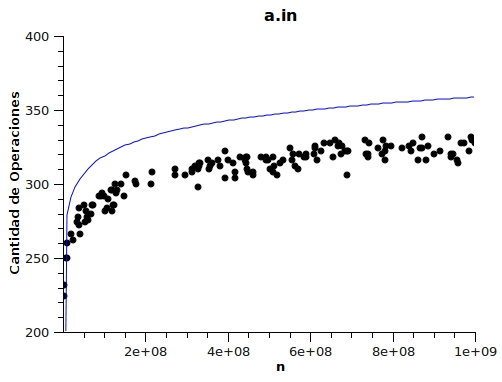
\includegraphics[scale = 0.5]{./../ej1/tests/a.jpg}[c] \hspace{30 pt}
%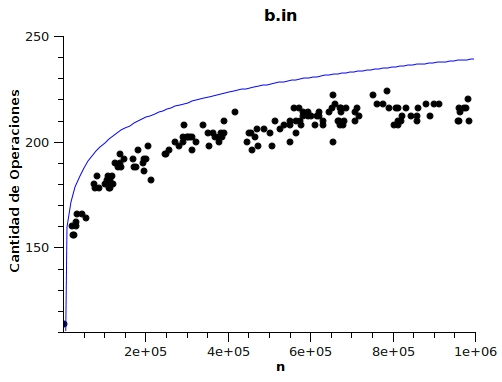
\includegraphics[scale = 0.5]{./../ej1/tests/b.jpg}[c] \\
%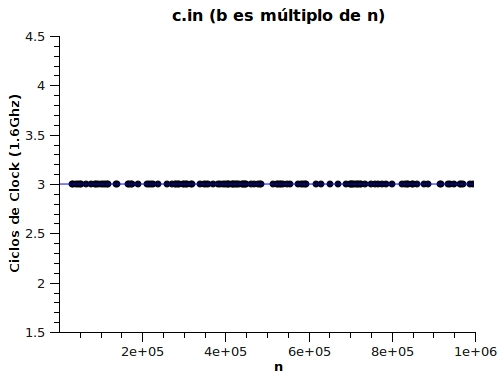
\includegraphics[scale = 0.5]{./../ej1/tests/c.jpg}[c] \hspace{30 pt}
%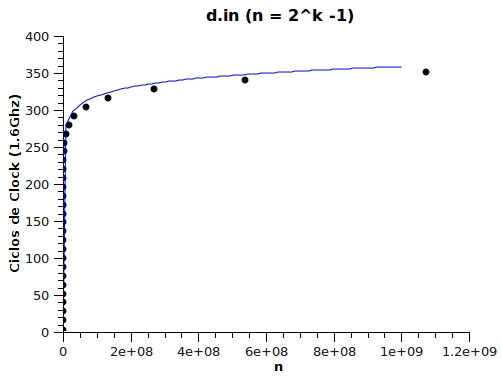
\includegraphics[scale = 0.5]{./../ej1/tests/d.jpg}[c] \\
%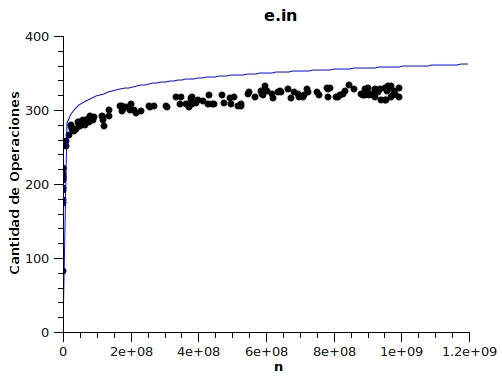
\includegraphics[scale = 0.5]{./../ej1/tests/e.jpg}[c] \hspace{30 pt}
%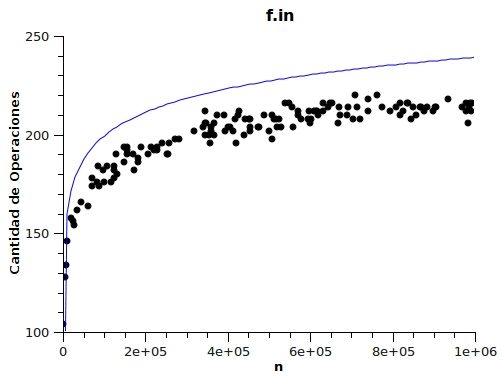
\includegraphics[scale = 0.5]{./../ej1/tests/f.jpg}[c] \\

%\subsection{Debate}
%\subsection{Comentarios}
%\subsection{Conclusiones}
